\documentclass[1p]{elsarticle_modified}
%\bibliographystyle{elsarticle-num}

%\usepackage[colorlinks]{hyperref}
%\usepackage{abbrmath_seonhwa} %\Abb, \Ascr, \Acal ,\Abf, \Afrak
\usepackage{amsfonts}
\usepackage{amssymb}
\usepackage{amsmath}
\usepackage{amsthm}
\usepackage{scalefnt}
\usepackage{amsbsy}
\usepackage{kotex}
\usepackage{caption}
\usepackage{subfig}
\usepackage{color}
\usepackage{graphicx}
\usepackage{xcolor} %% white, black, red, green, blue, cyan, magenta, yellow
\usepackage{float}
\usepackage{setspace}
\usepackage{hyperref}

\usepackage{tikz}
\usetikzlibrary{arrows}

\usepackage{multirow}
\usepackage{array} % fixed length table
\usepackage{hhline}

%%%%%%%%%%%%%%%%%%%%%
\makeatletter
\renewcommand*\env@matrix[1][\arraystretch]{%
	\edef\arraystretch{#1}%
	\hskip -\arraycolsep
	\let\@ifnextchar\new@ifnextchar
	\array{*\c@MaxMatrixCols c}}
\makeatother %https://tex.stackexchange.com/questions/14071/how-can-i-increase-the-line-spacing-in-a-matrix
%%%%%%%%%%%%%%%

\usepackage[normalem]{ulem}

\newcommand{\msout}[1]{\ifmmode\text{\sout{\ensuremath{#1}}}\else\sout{#1}\fi}
%SOURCE: \msout is \stkout macro in https://tex.stackexchange.com/questions/20609/strikeout-in-math-mode

\newcommand{\cancel}[1]{
	\ifmmode
	{\color{red}\msout{#1}}
	\else
	{\color{red}\sout{#1}}
	\fi
}

\newcommand{\add}[1]{
	{\color{blue}\uwave{#1}}
}

\newcommand{\replace}[2]{
	\ifmmode
	{\color{red}\msout{#1}}{\color{blue}\uwave{#2}}
	\else
	{\color{red}\sout{#1}}{\color{blue}\uwave{#2}}
	\fi
}

\newcommand{\Sol}{\mathcal{S}} %segment
\newcommand{\D}{D} %diagram
\newcommand{\A}{\mathcal{A}} %arc


%%%%%%%%%%%%%%%%%%%%%%%%%%%%%5 test

\def\sl{\operatorname{\textup{SL}}(2,\Cbb)}
\def\psl{\operatorname{\textup{PSL}}(2,\Cbb)}
\def\quan{\mkern 1mu \triangleright \mkern 1mu}

\theoremstyle{definition}
\newtheorem{thm}{Theorem}[section]
\newtheorem{prop}[thm]{Proposition}
\newtheorem{lem}[thm]{Lemma}
\newtheorem{ques}[thm]{Question}
\newtheorem{cor}[thm]{Corollary}
\newtheorem{defn}[thm]{Definition}
\newtheorem{exam}[thm]{Example}
\newtheorem{rmk}[thm]{Remark}
\newtheorem{alg}[thm]{Algorithm}

\newcommand{\I}{\sqrt{-1}}
\begin{document}

%\begin{frontmatter}
%
%\title{Boundary parabolic representations of knots up to 8 crossings}
%
%%% Group authors per affiliation:
%\author{Yunhi Cho} 
%\address{Department of Mathematics, University of Seoul, Seoul, Korea}
%\ead{yhcho@uos.ac.kr}
%
%
%\author{Seonhwa Kim} %\fnref{s_kim}}
%\address{Center for Geometry and Physics, Institute for Basic Science, Pohang, 37673, Korea}
%\ead{ryeona17@ibs.re.kr}
%
%\author{Hyuk Kim}
%\address{Department of Mathematical Sciences, Seoul National University, Seoul 08826, Korea}
%\ead{hyukkim@snu.ac.kr}
%
%\author{Seokbeom Yoon}
%\address{Department of Mathematical Sciences, Seoul National University, Seoul, 08826,  Korea}
%\ead{sbyoon15@snu.ac.kr}
%
%\begin{abstract}
%We find all boundary parabolic representation of knots up to 8 crossings.
%
%\end{abstract}
%\begin{keyword}
%    \MSC[2010] 57M25 
%\end{keyword}
%
%\end{frontmatter}

%\linenumbers
%\tableofcontents
%
\newcommand\colored[1]{\textcolor{white}{\rule[-0.35ex]{0.8em}{1.4ex}}\kern-0.8em\color{red} #1}%
%\newcommand\colored[1]{\textcolor{white}{ #1}\kern-2.17ex	\textcolor{white}{ #1}\kern-1.81ex	\textcolor{white}{ #1}\kern-2.15ex\color{red}#1	}

{\Large $\underline{12n_{0178}~(K12n_{0178})}$}

\setlength{\tabcolsep}{10pt}
\renewcommand{\arraystretch}{1.6}
\vspace{1cm}\begin{tabular}{m{100pt}>{\centering\arraybackslash}m{274pt}}
\multirow{5}{120pt}{
	\centering
	\includegraphics[width=112pt]{../../../GIT/diagram.site/Diagrams/png/2267_12n_0178.png}\\
\ \ \ A knot diagram\footnotemark}&
\allowdisplaybreaks
\textbf{Linearized knot diagam} \\
\cline{2-2}
 &
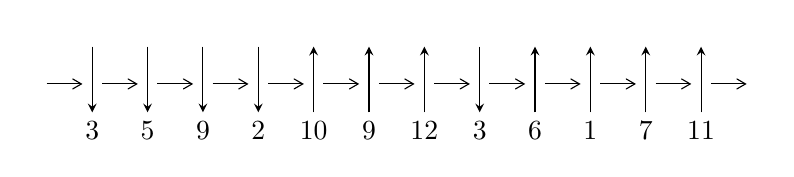
\begin{tikzpicture}[x=20pt, y=17pt]
	% nodes
	\node (C0) at (0, 0) {};
	\node (C1) at (1, 0) {};
	\node (C1U) at (1, +1) {};
	\node (C1D) at (1, -1) {3};

	\node (C2) at (2, 0) {};
	\node (C2U) at (2, +1) {};
	\node (C2D) at (2, -1) {5};

	\node (C3) at (3, 0) {};
	\node (C3U) at (3, +1) {};
	\node (C3D) at (3, -1) {9};

	\node (C4) at (4, 0) {};
	\node (C4U) at (4, +1) {};
	\node (C4D) at (4, -1) {2};

	\node (C5) at (5, 0) {};
	\node (C5U) at (5, +1) {};
	\node (C5D) at (5, -1) {10};

	\node (C6) at (6, 0) {};
	\node (C6U) at (6, +1) {};
	\node (C6D) at (6, -1) {9};

	\node (C7) at (7, 0) {};
	\node (C7U) at (7, +1) {};
	\node (C7D) at (7, -1) {12};

	\node (C8) at (8, 0) {};
	\node (C8U) at (8, +1) {};
	\node (C8D) at (8, -1) {3};

	\node (C9) at (9, 0) {};
	\node (C9U) at (9, +1) {};
	\node (C9D) at (9, -1) {6};

	\node (C10) at (10, 0) {};
	\node (C10U) at (10, +1) {};
	\node (C10D) at (10, -1) {1};

	\node (C11) at (11, 0) {};
	\node (C11U) at (11, +1) {};
	\node (C11D) at (11, -1) {7};

	\node (C12) at (12, 0) {};
	\node (C12U) at (12, +1) {};
	\node (C12D) at (12, -1) {11};
	\node (C13) at (13, 0) {};

	% arrows
	\draw[->,>={angle 60}]
	(C0) edge (C1) (C1) edge (C2) (C2) edge (C3) (C3) edge (C4) (C4) edge (C5) (C5) edge (C6) (C6) edge (C7) (C7) edge (C8) (C8) edge (C9) (C9) edge (C10) (C10) edge (C11) (C11) edge (C12) (C12) edge (C13) ;	\draw[->,>=stealth]
	(C1U) edge (C1D) (C2U) edge (C2D) (C3U) edge (C3D) (C4U) edge (C4D) (C5D) edge (C5U) (C6D) edge (C6U) (C7D) edge (C7U) (C8U) edge (C8D) (C9D) edge (C9U) (C10D) edge (C10U) (C11D) edge (C11U) (C12D) edge (C12U) ;
	\end{tikzpicture} \\
\hhline{~~} \\& 
\textbf{Solving Sequence} \\ \cline{2-2} 
 &
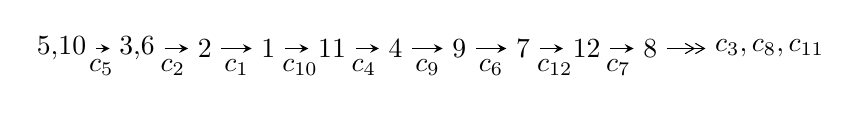
\begin{tikzpicture}[x=23pt, y=7pt]
	% node
	\node (A0) at (-1/8, 0) {5,10};
	\node (A1) at (17/16, 0) {3,6};
	\node (A2) at (17/8, 0) {2};
	\node (A3) at (25/8, 0) {1};
	\node (A4) at (33/8, 0) {11};
	\node (A5) at (41/8, 0) {4};
	\node (A6) at (49/8, 0) {9};
	\node (A7) at (57/8, 0) {7};
	\node (A8) at (65/8, 0) {12};
	\node (A9) at (73/8, 0) {8};
	\node (C1) at (1/2, -1) {$c_{5}$};
	\node (C2) at (13/8, -1) {$c_{2}$};
	\node (C3) at (21/8, -1) {$c_{1}$};
	\node (C4) at (29/8, -1) {$c_{10}$};
	\node (C5) at (37/8, -1) {$c_{4}$};
	\node (C6) at (45/8, -1) {$c_{9}$};
	\node (C7) at (53/8, -1) {$c_{6}$};
	\node (C8) at (61/8, -1) {$c_{12}$};
	\node (C9) at (69/8, -1) {$c_{7}$};
	\node (A10) at (11, 0) {$c_{3},c_{8},c_{11}$};

	% edge
	\draw[->,>=stealth]	
	(A0) edge (A1) (A1) edge (A2) (A2) edge (A3) (A3) edge (A4) (A4) edge (A5) (A5) edge (A6) (A6) edge (A7) (A7) edge (A8) (A8) edge (A9) ;
	\draw[->>,>={angle 60}]	
	(A9) edge (A10);
\end{tikzpicture} \\ 

\end{tabular} \\

\footnotetext{
The image of knot diagram is generated by the software ``\textbf{Draw programme}" developed by Andrew Bartholomew(\url{http://www.layer8.co.uk/maths/draw/index.htm\#Running-draw}), where we modified some parts for our purpose(\url{https://github.com/CATsTAILs/LinksPainter}).
}\phantom \\ \newline 
\centering \textbf{Ideals for irreducible components\footnotemark of $X_{\text{par}}$} 
 
\begin{align*}
I^u_{1}&=\langle 
9.57275\times10^{53} u^{54}+1.47300\times10^{54} u^{53}+\cdots+8.10588\times10^{54} b+5.80479\times10^{54},\\
\phantom{I^u_{1}}&\phantom{= \langle  }-1.30447\times10^{55} u^{54}-2.66313\times10^{55} u^{53}+\cdots+8.10588\times10^{54} a-2.06989\times10^{55},\;u^{55}+2 u^{54}+\cdots+4 u+1\rangle \\
I^u_{2}&=\langle 
b+1,\;- u^3- u^2+a-3 u-2,\;u^5+u^4+4 u^3+3 u^2+3 u+1\rangle \\
\\
\end{align*}
\raggedright * 2 irreducible components of $\dim_{\mathbb{C}}=0$, with total 60 representations.\\
\footnotetext{All coefficients of polynomials are rational numbers. But the coefficients are sometimes approximated in decimal forms when there is not enough margin.}
\newpage
\renewcommand{\arraystretch}{1}
\centering \section*{I. $I^u_{1}= \langle 9.57\times10^{53} u^{54}+1.47\times10^{54} u^{53}+\cdots+8.11\times10^{54} b+5.80\times10^{54},\;-1.30\times10^{55} u^{54}-2.66\times10^{55} u^{53}+\cdots+8.11\times10^{54} a-2.07\times10^{55},\;u^{55}+2 u^{54}+\cdots+4 u+1 \rangle$}
\flushleft \textbf{(i) Arc colorings}\\
\begin{tabular}{m{7pt} m{180pt} m{7pt} m{180pt} }
\flushright $a_{5}=$&$\begin{pmatrix}1\\0\end{pmatrix}$ \\
\flushright $a_{10}=$&$\begin{pmatrix}0\\u\end{pmatrix}$ \\
\flushright $a_{3}=$&$\begin{pmatrix}1.60929 u^{54}+3.28543 u^{53}+\cdots-0.667235 u+2.55356\\-0.118096 u^{54}-0.181720 u^{53}+\cdots+1.32185 u-0.716120\end{pmatrix}$ \\
\flushright $a_{6}=$&$\begin{pmatrix}1\\- u^2\end{pmatrix}$ \\
\flushright $a_{2}=$&$\begin{pmatrix}1.49119 u^{54}+3.10371 u^{53}+\cdots+0.654617 u+1.83744\\-0.118096 u^{54}-0.181720 u^{53}+\cdots+1.32185 u-0.716120\end{pmatrix}$ \\
\flushright $a_{1}=$&$\begin{pmatrix}0.0670214 u^{54}+0.408100 u^{53}+\cdots+0.231214 u-0.865681\\-0.119667 u^{54}-0.280385 u^{53}+\cdots+1.25999 u+0.229470\end{pmatrix}$ \\
\flushright $a_{11}=$&$\begin{pmatrix}-0.0627514 u^{54}+0.225048 u^{53}+\cdots+2.67144 u+0.447681\\-0.115045 u^{54}-0.310044 u^{53}+\cdots+1.95308 u+0.125113\end{pmatrix}$ \\
\flushright $a_{4}=$&$\begin{pmatrix}1.55763 u^{54}+3.14463 u^{53}+\cdots-0.402533 u+2.59906\\-0.0743860 u^{54}-0.0787220 u^{53}+\cdots+0.855578 u-0.799104\end{pmatrix}$ \\
\flushright $a_{9}=$&$\begin{pmatrix}- u\\u^3+u\end{pmatrix}$ \\
\flushright $a_{7}=$&$\begin{pmatrix}u^2+1\\- u^4-2 u^2\end{pmatrix}$ \\
\flushright $a_{12}=$&$\begin{pmatrix}-0.451706 u^{54}-0.711582 u^{53}+\cdots+5.15586 u+0.621849\\0.0254744 u^{54}-0.291495 u^{53}+\cdots-0.656683 u-0.382675\end{pmatrix}$ \\
\flushright $a_{8}=$&$\begin{pmatrix}0.00353609 u^{54}-0.0598773 u^{53}+\cdots-2.34653 u+0.394759\\0.0754811 u^{54}+0.239141 u^{53}+\cdots+0.161367 u-0.119595\end{pmatrix}$\\&\end{tabular}
\flushleft \textbf{(ii) Obstruction class $= -1$}\\~\\
\flushleft \textbf{(iii) Cusp Shapes $= -4.76753 u^{54}+0.155153 u^{53}+\cdots+63.8827 u+5.20939$}\\~\\
\newpage\renewcommand{\arraystretch}{1}
\flushleft \textbf{(iv) u-Polynomials at the component}\newline \\
\begin{tabular}{m{50pt}|m{274pt}}
Crossings & \hspace{64pt}u-Polynomials at each crossing \\
\hline $$\begin{aligned}c_{1}\end{aligned}$$&$\begin{aligned}
&u^{55}+24 u^{54}+\cdots-40 u+1
\end{aligned}$\\
\hline $$\begin{aligned}c_{2},c_{4}\end{aligned}$$&$\begin{aligned}
&u^{55}-6 u^{54}+\cdots+12 u+1
\end{aligned}$\\
\hline $$\begin{aligned}c_{3},c_{8}\end{aligned}$$&$\begin{aligned}
&u^{55}+u^{54}+\cdots+448 u+32
\end{aligned}$\\
\hline $$\begin{aligned}c_{5},c_{6},c_{9}\end{aligned}$$&$\begin{aligned}
&u^{55}+2 u^{54}+\cdots+4 u+1
\end{aligned}$\\
\hline $$\begin{aligned}c_{7},c_{11}\end{aligned}$$&$\begin{aligned}
&u^{55}+2 u^{54}+\cdots+4 u+1
\end{aligned}$\\
\hline $$\begin{aligned}c_{10},c_{12}\end{aligned}$$&$\begin{aligned}
&u^{55}-20 u^{54}+\cdots+22 u-1
\end{aligned}$\\
\hline
\end{tabular}\\~\\
\newpage\renewcommand{\arraystretch}{1}
\flushleft \textbf{(v) Riley Polynomials at the component}\newline \\
\begin{tabular}{m{50pt}|m{274pt}}
Crossings & \hspace{64pt}Riley Polynomials at each crossing \\
\hline $$\begin{aligned}c_{1}\end{aligned}$$&$\begin{aligned}
&y^{55}+20 y^{54}+\cdots-40060 y-1
\end{aligned}$\\
\hline $$\begin{aligned}c_{2},c_{4}\end{aligned}$$&$\begin{aligned}
&y^{55}-24 y^{54}+\cdots-40 y-1
\end{aligned}$\\
\hline $$\begin{aligned}c_{3},c_{8}\end{aligned}$$&$\begin{aligned}
&y^{55}+33 y^{54}+\cdots+27136 y-1024
\end{aligned}$\\
\hline $$\begin{aligned}c_{5},c_{6},c_{9}\end{aligned}$$&$\begin{aligned}
&y^{55}+44 y^{54}+\cdots+22 y-1
\end{aligned}$\\
\hline $$\begin{aligned}c_{7},c_{11}\end{aligned}$$&$\begin{aligned}
&y^{55}-20 y^{54}+\cdots+22 y-1
\end{aligned}$\\
\hline $$\begin{aligned}c_{10},c_{12}\end{aligned}$$&$\begin{aligned}
&y^{55}+32 y^{54}+\cdots+210 y-1
\end{aligned}$\\
\hline
\end{tabular}\\~\\
\newpage\flushleft \textbf{(vi) Complex Volumes and Cusp Shapes}
$$\begin{array}{c|c|c}  
\text{Solutions to }I^u_{1}& \I (\text{vol} + \sqrt{-1}CS) & \text{Cusp shape}\\
 \hline 
\begin{aligned}
u &= \phantom{-}0.072313 + 0.999634 I \\
a &= \phantom{-}2.29927 - 6.60365 I \\
b &= -0.958174 - 0.009887 I\end{aligned}
 & -3.21384 - 2.03983 I & -44.2012 - 7.6598 I \\ \hline\begin{aligned}
u &= \phantom{-}0.072313 - 0.999634 I \\
a &= \phantom{-}2.29927 + 6.60365 I \\
b &= -0.958174 + 0.009887 I\end{aligned}
 & -3.21384 + 2.03983 I & -44.2012 + 7.6598 I \\ \hline\begin{aligned}
u &= \phantom{-}0.993934 + 0.162352 I \\
a &= -0.493168 + 1.055260 I \\
b &= \phantom{-}1.033280 - 0.648823 I\end{aligned}
 & \phantom{-}0.91067 + 4.40051 I & \phantom{-}0.64951 - 3.45726 I \\ \hline\begin{aligned}
u &= \phantom{-}0.993934 - 0.162352 I \\
a &= -0.493168 - 1.055260 I \\
b &= \phantom{-}1.033280 + 0.648823 I\end{aligned}
 & \phantom{-}0.91067 - 4.40051 I & \phantom{-}0.64951 + 3.45726 I \\ \hline\begin{aligned}
u &= -1.001870 + 0.130107 I \\
a &= -0.620284 - 1.134160 I \\
b &= \phantom{-}1.114800 + 0.710314 I\end{aligned}
 & \phantom{-}2.39213 - 10.23010 I & \phantom{-}2.28495 + 7.44906 I \\ \hline\begin{aligned}
u &= -1.001870 - 0.130107 I \\
a &= -0.620284 + 1.134160 I \\
b &= \phantom{-}1.114800 - 0.710314 I\end{aligned}
 & \phantom{-}2.39213 + 10.23010 I & \phantom{-}2.28495 - 7.44906 I \\ \hline\begin{aligned}
u &= \phantom{-}0.137708 + 0.978085 I \\
a &= \phantom{-}0.876327 - 0.305252 I \\
b &= -0.0541745 + 0.0630040 I\end{aligned}
 & -1.78463 + 2.08708 I & -0.67506 - 3.94082 I \\ \hline\begin{aligned}
u &= \phantom{-}0.137708 - 0.978085 I \\
a &= \phantom{-}0.876327 + 0.305252 I \\
b &= -0.0541745 - 0.0630040 I\end{aligned}
 & -1.78463 - 2.08708 I & -0.67506 + 3.94082 I \\ \hline\begin{aligned}
u &= -0.920019 + 0.123504 I \\
a &= -0.295321 - 1.372000 I \\
b &= \phantom{-}0.879379 + 0.854012 I\end{aligned}
 & \phantom{-}7.49655 - 3.13489 I & \phantom{-}7.28291 + 3.22695 I \\ \hline\begin{aligned}
u &= -0.920019 - 0.123504 I \\
a &= -0.295321 + 1.372000 I \\
b &= \phantom{-}0.879379 - 0.854012 I\end{aligned}
 & \phantom{-}7.49655 + 3.13489 I & \phantom{-}7.28291 - 3.22695 I\\
 \hline 
 \end{array}$$\newpage$$\begin{array}{c|c|c}  
\text{Solutions to }I^u_{1}& \I (\text{vol} + \sqrt{-1}CS) & \text{Cusp shape}\\
 \hline 
\begin{aligned}
u &= \phantom{-}0.210457 + 1.111180 I \\
a &= \phantom{-}0.166418 - 1.112530 I \\
b &= -0.533647 + 0.528199 I\end{aligned}
 & -1.62268 + 2.42881 I & \phantom{-0.000000 } 0 \\ \hline\begin{aligned}
u &= \phantom{-}0.210457 - 1.111180 I \\
a &= \phantom{-}0.166418 + 1.112530 I \\
b &= -0.533647 - 0.528199 I\end{aligned}
 & -1.62268 - 2.42881 I & \phantom{-0.000000 } 0 \\ \hline\begin{aligned}
u &= -0.085057 + 1.147710 I \\
a &= -0.91778 + 1.25610 I \\
b &= -1.132530 - 0.298762 I\end{aligned}
 & -4.28823 - 1.16800 I & \phantom{-0.000000 } 0 \\ \hline\begin{aligned}
u &= -0.085057 - 1.147710 I \\
a &= -0.91778 - 1.25610 I \\
b &= -1.132530 + 0.298762 I\end{aligned}
 & -4.28823 + 1.16800 I & \phantom{-0.000000 } 0 \\ \hline\begin{aligned}
u &= \phantom{-}0.828480 + 0.174420 I \\
a &= \phantom{-}0.110067 + 1.220490 I \\
b &= \phantom{-}0.608202 - 0.730301 I\end{aligned}
 & \phantom{-}2.20429 + 0.89304 I & \phantom{-}2.75128 - 2.60461 I \\ \hline\begin{aligned}
u &= \phantom{-}0.828480 - 0.174420 I \\
a &= \phantom{-}0.110067 - 1.220490 I \\
b &= \phantom{-}0.608202 + 0.730301 I\end{aligned}
 & \phantom{-}2.20429 - 0.89304 I & \phantom{-}2.75128 + 2.60461 I \\ \hline\begin{aligned}
u &= -0.819216 + 0.097633 I \\
a &= \phantom{-}0.17500 - 1.53413 I \\
b &= \phantom{-}0.550668 + 0.941243 I\end{aligned}
 & \phantom{-}4.13978 + 4.18210 I & \phantom{-}5.23081 - 2.78874 I \\ \hline\begin{aligned}
u &= -0.819216 - 0.097633 I \\
a &= \phantom{-}0.17500 + 1.53413 I \\
b &= \phantom{-}0.550668 - 0.941243 I\end{aligned}
 & \phantom{-}4.13978 - 4.18210 I & \phantom{-}5.23081 + 2.78874 I \\ \hline\begin{aligned}
u &= -0.146957 + 1.227320 I \\
a &= -0.250773 + 0.958708 I \\
b &= -1.25230 - 0.85045 I\end{aligned}
 & -5.99858 - 1.47280 I & \phantom{-0.000000 } 0 \\ \hline\begin{aligned}
u &= -0.146957 - 1.227320 I \\
a &= -0.250773 - 0.958708 I \\
b &= -1.25230 + 0.85045 I\end{aligned}
 & -5.99858 + 1.47280 I & \phantom{-0.000000 } 0\\
 \hline 
 \end{array}$$\newpage$$\begin{array}{c|c|c}  
\text{Solutions to }I^u_{1}& \I (\text{vol} + \sqrt{-1}CS) & \text{Cusp shape}\\
 \hline 
\begin{aligned}
u &= \phantom{-}0.381441 + 1.177740 I \\
a &= -0.265339 - 0.556912 I \\
b &= \phantom{-}0.209231 + 1.073740 I\end{aligned}
 & -0.86862 + 3.44583 I & \phantom{-0.000000 } 0 \\ \hline\begin{aligned}
u &= \phantom{-}0.381441 - 1.177740 I \\
a &= -0.265339 + 0.556912 I \\
b &= \phantom{-}0.209231 - 1.073740 I\end{aligned}
 & -0.86862 - 3.44583 I & \phantom{-0.000000 } 0 \\ \hline\begin{aligned}
u &= \phantom{-}0.177845 + 1.232580 I \\
a &= -0.197287 - 0.999523 I \\
b &= -1.11540 + 1.02762 I\end{aligned}
 & -5.34328 + 6.53526 I & \phantom{-0.000000 } 0 \\ \hline\begin{aligned}
u &= \phantom{-}0.177845 - 1.232580 I \\
a &= -0.197287 + 0.999523 I \\
b &= -1.11540 - 1.02762 I\end{aligned}
 & -5.34328 - 6.53526 I & \phantom{-0.000000 } 0 \\ \hline\begin{aligned}
u &= -0.014389 + 1.247610 I \\
a &= -0.396154 + 0.123893 I \\
b &= -1.75259 - 0.09946 I\end{aligned}
 & -7.40193 - 2.54973 I & \phantom{-0.000000 } 0 \\ \hline\begin{aligned}
u &= -0.014389 - 1.247610 I \\
a &= -0.396154 - 0.123893 I \\
b &= -1.75259 + 0.09946 I\end{aligned}
 & -7.40193 + 2.54973 I & \phantom{-0.000000 } 0 \\ \hline\begin{aligned}
u &= \phantom{-}0.614835 + 1.102710 I \\
a &= -0.145574 + 0.034160 I \\
b &= \phantom{-}0.742661 + 0.465384 I\end{aligned}
 & -1.99257 + 1.17321 I & \phantom{-0.000000 } 0 \\ \hline\begin{aligned}
u &= \phantom{-}0.614835 - 1.102710 I \\
a &= -0.145574 - 0.034160 I \\
b &= \phantom{-}0.742661 - 0.465384 I\end{aligned}
 & -1.99257 - 1.17321 I & \phantom{-0.000000 } 0 \\ \hline\begin{aligned}
u &= -0.468976 + 1.184810 I \\
a &= -0.356235 + 0.277549 I \\
b &= \phantom{-}0.611745 - 0.951185 I\end{aligned}
 & \phantom{-}4.23996 - 1.81305 I & \phantom{-0.000000 } 0 \\ \hline\begin{aligned}
u &= -0.468976 - 1.184810 I \\
a &= -0.356235 - 0.277549 I \\
b &= \phantom{-}0.611745 + 0.951185 I\end{aligned}
 & \phantom{-}4.23996 + 1.81305 I & \phantom{-0.000000 } 0\\
 \hline 
 \end{array}$$\newpage$$\begin{array}{c|c|c}  
\text{Solutions to }I^u_{1}& \I (\text{vol} + \sqrt{-1}CS) & \text{Cusp shape}\\
 \hline 
\begin{aligned}
u &= -0.394816 + 1.214720 I \\
a &= -0.407055 + 0.558974 I \\
b &= \phantom{-}0.327121 - 1.259930 I\end{aligned}
 & \phantom{-}0.69756 - 8.56499 I & \phantom{-0.000000 } 0 \\ \hline\begin{aligned}
u &= -0.394816 - 1.214720 I \\
a &= -0.407055 - 0.558974 I \\
b &= \phantom{-}0.327121 + 1.259930 I\end{aligned}
 & \phantom{-}0.69756 + 8.56499 I & \phantom{-0.000000 } 0 \\ \hline\begin{aligned}
u &= -0.601783 + 1.184100 I \\
a &= -0.280221 - 0.060494 I \\
b &= \phantom{-}0.893170 - 0.577080 I\end{aligned}
 & -0.82436 + 4.63316 I & \phantom{-0.000000 } 0 \\ \hline\begin{aligned}
u &= -0.601783 - 1.184100 I \\
a &= -0.280221 + 0.060494 I \\
b &= \phantom{-}0.893170 + 0.577080 I\end{aligned}
 & -0.82436 - 4.63316 I & \phantom{-0.000000 } 0 \\ \hline\begin{aligned}
u &= -0.33663 + 1.38775 I \\
a &= \phantom{-}0.970187 - 0.767712 I \\
b &= \phantom{-}0.813537 + 0.578538 I\end{aligned}
 & -0.568084 + 0.034758 I & \phantom{-0.000000 } 0 \\ \hline\begin{aligned}
u &= -0.33663 - 1.38775 I \\
a &= \phantom{-}0.970187 + 0.767712 I \\
b &= \phantom{-}0.813537 - 0.578538 I\end{aligned}
 & -0.568084 - 0.034758 I & \phantom{-0.000000 } 0 \\ \hline\begin{aligned}
u &= -0.42146 + 1.38024 I \\
a &= \phantom{-}0.787185 - 1.119040 I \\
b &= \phantom{-}1.083980 + 0.732016 I\end{aligned}
 & \phantom{-}2.75927 - 7.95467 I & \phantom{-0.000000 } 0 \\ \hline\begin{aligned}
u &= -0.42146 - 1.38024 I \\
a &= \phantom{-}0.787185 + 1.119040 I \\
b &= \phantom{-}1.083980 - 0.732016 I\end{aligned}
 & \phantom{-}2.75927 + 7.95467 I & \phantom{-0.000000 } 0 \\ \hline\begin{aligned}
u &= -0.46185 + 1.38681 I \\
a &= \phantom{-}0.562764 - 1.256260 I \\
b &= \phantom{-}1.29657 + 0.72034 I\end{aligned}
 & -2.3616 - 15.4470 I & \phantom{-0.000000 } 0 \\ \hline\begin{aligned}
u &= -0.46185 - 1.38681 I \\
a &= \phantom{-}0.562764 + 1.256260 I \\
b &= \phantom{-}1.29657 - 0.72034 I\end{aligned}
 & -2.3616 + 15.4470 I & \phantom{-0.000000 } 0\\
 \hline 
 \end{array}$$\newpage$$\begin{array}{c|c|c}  
\text{Solutions to }I^u_{1}& \I (\text{vol} + \sqrt{-1}CS) & \text{Cusp shape}\\
 \hline 
\begin{aligned}
u &= \phantom{-}0.45518 + 1.39872 I \\
a &= \phantom{-}0.558722 + 1.163830 I \\
b &= \phantom{-}1.25544 - 0.65692 I\end{aligned}
 & -3.98197 + 9.57742 I & \phantom{-0.000000 } 0 \\ \hline\begin{aligned}
u &= \phantom{-}0.45518 - 1.39872 I \\
a &= \phantom{-}0.558722 - 1.163830 I \\
b &= \phantom{-}1.25544 + 0.65692 I\end{aligned}
 & -3.98197 - 9.57742 I & \phantom{-0.000000 } 0 \\ \hline\begin{aligned}
u &= \phantom{-}0.38456 + 1.42439 I \\
a &= \phantom{-}0.750991 + 0.847131 I \\
b &= \phantom{-}0.988852 - 0.539464 I\end{aligned}
 & -2.92074 + 5.31715 I & \phantom{-0.000000 } 0 \\ \hline\begin{aligned}
u &= \phantom{-}0.38456 - 1.42439 I \\
a &= \phantom{-}0.750991 - 0.847131 I \\
b &= \phantom{-}0.988852 + 0.539464 I\end{aligned}
 & -2.92074 - 5.31715 I & \phantom{-0.000000 } 0 \\ \hline\begin{aligned}
u &= \phantom{-}0.443695 + 0.152031 I \\
a &= \phantom{-}2.39257 - 1.10066 I \\
b &= -0.785702 + 0.556656 I\end{aligned}
 & -1.28934 + 4.28381 I & \phantom{-}2.06004 - 6.33313 I \\ \hline\begin{aligned}
u &= \phantom{-}0.443695 - 0.152031 I \\
a &= \phantom{-}2.39257 + 1.10066 I \\
b &= -0.785702 - 0.556656 I\end{aligned}
 & -1.28934 - 4.28381 I & \phantom{-}2.06004 + 6.33313 I \\ \hline\begin{aligned}
u &= \phantom{-}0.458210 + 0.088205 I \\
a &= \phantom{-}1.25519 + 0.67781 I \\
b &= -0.128180 - 0.374679 I\end{aligned}
 & \phantom{-}1.217180 + 0.208314 I & \phantom{-}8.43782 - 0.43348 I \\ \hline\begin{aligned}
u &= \phantom{-}0.458210 - 0.088205 I \\
a &= \phantom{-}1.25519 - 0.67781 I \\
b &= -0.128180 + 0.374679 I\end{aligned}
 & \phantom{-}1.217180 - 0.208314 I & \phantom{-}8.43782 + 0.43348 I \\ \hline\begin{aligned}
u &= -0.359115 + 0.183471 I \\
a &= \phantom{-}2.71826 + 0.82408 I \\
b &= -0.926073 - 0.380961 I\end{aligned}
 & -1.94814 + 0.37120 I & -0.242965 - 0.911940 I \\ \hline\begin{aligned}
u &= -0.359115 - 0.183471 I \\
a &= \phantom{-}2.71826 - 0.82408 I \\
b &= -0.926073 + 0.380961 I\end{aligned}
 & -1.94814 - 0.37120 I & -0.242965 + 0.911940 I\\
 \hline 
 \end{array}$$\newpage$$\begin{array}{c|c|c}  
\text{Solutions to }I^u_{1}& \I (\text{vol} + \sqrt{-1}CS) & \text{Cusp shape}\\
 \hline 
\begin{aligned}
u &= -0.069012 + 0.377349 I \\
a &= \phantom{-}3.57577 + 0.18002 I \\
b &= -1.196500 - 0.044788 I\end{aligned}
 & -2.88229 - 2.31843 I & \phantom{-}4.89435 + 2.66761 I \\ \hline\begin{aligned}
u &= -0.069012 - 0.377349 I \\
a &= \phantom{-}3.57577 - 0.18002 I \\
b &= -1.196500 + 0.044788 I\end{aligned}
 & -2.88229 + 2.31843 I & \phantom{-}4.89435 - 2.66761 I \\ \hline\begin{aligned}
u &= \phantom{-}0.05440 + 1.73056 I \\
a &= \phantom{-}0.565358 + 0.054624 I \\
b &= \phantom{-}0.867697 - 0.027497 I\end{aligned}
 & -12.32020 + 3.39229 I & \phantom{-0.000000 } 0 \\ \hline\begin{aligned}
u &= \phantom{-}0.05440 - 1.73056 I \\
a &= \phantom{-}0.565358 - 0.054624 I \\
b &= \phantom{-}0.867697 + 0.027497 I\end{aligned}
 & -12.32020 - 3.39229 I & \phantom{-0.000000 } 0 \\ \hline\begin{aligned}
u &= -0.223807\phantom{ +0.000000I} \\
a &= \phantom{-}2.72223\phantom{ +0.000000I} \\
b &= -0.882156\phantom{ +0.000000I}\end{aligned}
 & -1.26969\phantom{ +0.000000I} & -9.83510\phantom{ +0.000000I}\\
 \hline 
 \end{array}$$\newpage\newpage\renewcommand{\arraystretch}{1}
\centering \section*{II. $I^u_{2}= \langle b+1,\;- u^3- u^2+a-3 u-2,\;u^5+u^4+4 u^3+3 u^2+3 u+1 \rangle$}
\flushleft \textbf{(i) Arc colorings}\\
\begin{tabular}{m{7pt} m{180pt} m{7pt} m{180pt} }
\flushright $a_{5}=$&$\begin{pmatrix}1\\0\end{pmatrix}$ \\
\flushright $a_{10}=$&$\begin{pmatrix}0\\u\end{pmatrix}$ \\
\flushright $a_{3}=$&$\begin{pmatrix}u^3+u^2+3 u+2\\-1\end{pmatrix}$ \\
\flushright $a_{6}=$&$\begin{pmatrix}1\\- u^2\end{pmatrix}$ \\
\flushright $a_{2}=$&$\begin{pmatrix}u^3+u^2+3 u+1\\-1\end{pmatrix}$ \\
\flushright $a_{1}=$&$\begin{pmatrix}-1\\0\end{pmatrix}$ \\
\flushright $a_{11}=$&$\begin{pmatrix}u\\u\end{pmatrix}$ \\
\flushright $a_{4}=$&$\begin{pmatrix}u^3+u^2+3 u+2\\-1\end{pmatrix}$ \\
\flushright $a_{9}=$&$\begin{pmatrix}- u\\u^3+u\end{pmatrix}$ \\
\flushright $a_{7}=$&$\begin{pmatrix}u^2+1\\- u^4-2 u^2\end{pmatrix}$ \\
\flushright $a_{12}=$&$\begin{pmatrix}- u^2-1\\- u^2\end{pmatrix}$ \\
\flushright $a_{8}=$&$\begin{pmatrix}- u\\u^3+u\end{pmatrix}$\\&\end{tabular}
\flushleft \textbf{(ii) Obstruction class $= 1$}\\~\\
\flushleft \textbf{(iii) Cusp Shapes $= 4 u^4+3 u^3+20 u^2+8 u+8$}\\~\\
\newpage\renewcommand{\arraystretch}{1}
\flushleft \textbf{(iv) u-Polynomials at the component}\newline \\
\begin{tabular}{m{50pt}|m{274pt}}
Crossings & \hspace{64pt}u-Polynomials at each crossing \\
\hline $$\begin{aligned}c_{1},c_{2}\end{aligned}$$&$\begin{aligned}
&(u-1)^5
\end{aligned}$\\
\hline $$\begin{aligned}c_{3},c_{8}\end{aligned}$$&$\begin{aligned}
&u^5
\end{aligned}$\\
\hline $$\begin{aligned}c_{4}\end{aligned}$$&$\begin{aligned}
&(u+1)^5
\end{aligned}$\\
\hline $$\begin{aligned}c_{5},c_{6},c_{10}\end{aligned}$$&$\begin{aligned}
&u^5+u^4+4 u^3+3 u^2+3 u+1
\end{aligned}$\\
\hline $$\begin{aligned}c_{7}\end{aligned}$$&$\begin{aligned}
&u^5+u^4- u^2+u+1
\end{aligned}$\\
\hline $$\begin{aligned}c_{9},c_{12}\end{aligned}$$&$\begin{aligned}
&u^5- u^4+4 u^3-3 u^2+3 u-1
\end{aligned}$\\
\hline $$\begin{aligned}c_{11}\end{aligned}$$&$\begin{aligned}
&u^5- u^4+u^2+u-1
\end{aligned}$\\
\hline
\end{tabular}\\~\\
\newpage\renewcommand{\arraystretch}{1}
\flushleft \textbf{(v) Riley Polynomials at the component}\newline \\
\begin{tabular}{m{50pt}|m{274pt}}
Crossings & \hspace{64pt}Riley Polynomials at each crossing \\
\hline $$\begin{aligned}c_{1},c_{2},c_{4}\end{aligned}$$&$\begin{aligned}
&(y-1)^5
\end{aligned}$\\
\hline $$\begin{aligned}c_{3},c_{8}\end{aligned}$$&$\begin{aligned}
&y^5
\end{aligned}$\\
\hline $$\begin{aligned}c_{5},c_{6},c_{9}\\c_{10},c_{12}\end{aligned}$$&$\begin{aligned}
&y^5+7 y^4+16 y^3+13 y^2+3 y-1
\end{aligned}$\\
\hline $$\begin{aligned}c_{7},c_{11}\end{aligned}$$&$\begin{aligned}
&y^5- y^4+4 y^3-3 y^2+3 y-1
\end{aligned}$\\
\hline
\end{tabular}\\~\\
\newpage\flushleft \textbf{(vi) Complex Volumes and Cusp Shapes}
$$\begin{array}{c|c|c}  
\text{Solutions to }I^u_{2}& \I (\text{vol} + \sqrt{-1}CS) & \text{Cusp shape}\\
 \hline 
\begin{aligned}
u &= -0.233677 + 0.885557 I \\
a &= \phantom{-}1.10636 + 1.69341 I \\
b &= -1.00000\phantom{ +0.000000I}\end{aligned}
 & -3.46474 - 2.21397 I & -5.40639 - 0.42541 I \\ \hline\begin{aligned}
u &= -0.233677 - 0.885557 I \\
a &= \phantom{-}1.10636 - 1.69341 I \\
b &= -1.00000\phantom{ +0.000000I}\end{aligned}
 & -3.46474 + 2.21397 I & -5.40639 + 0.42541 I \\ \hline\begin{aligned}
u &= -0.416284\phantom{ +0.000000I} \\
a &= \phantom{-}0.852303\phantom{ +0.000000I} \\
b &= -1.00000\phantom{ +0.000000I}\end{aligned}
 & -0.762751\phantom{ +0.000000I} & \phantom{-}8.03930\phantom{ +0.000000I} \\ \hline\begin{aligned}
u &= -0.05818 + 1.69128 I \\
a &= -0.532511 + 0.056433 I \\
b &= -1.00000\phantom{ +0.000000I}\end{aligned}
 & -12.60320 - 3.33174 I & -15.6132 - 0.3694 I \\ \hline\begin{aligned}
u &= -0.05818 - 1.69128 I \\
a &= -0.532511 - 0.056433 I \\
b &= -1.00000\phantom{ +0.000000I}\end{aligned}
 & -12.60320 + 3.33174 I & -15.6132 + 0.3694 I\\
 \hline 
 \end{array}$$\newpage
\newpage\renewcommand{\arraystretch}{1}
\centering \section*{ III. u-Polynomials}
\begin{tabular}{m{50pt}|m{274pt}}
Crossings & \hspace{64pt}u-Polynomials at each crossing \\
\hline $$\begin{aligned}c_{1}\end{aligned}$$&$\begin{aligned}
&((u-1)^5)(u^{55}+24 u^{54}+\cdots-40 u+1)
\end{aligned}$\\
\hline $$\begin{aligned}c_{2}\end{aligned}$$&$\begin{aligned}
&((u-1)^5)(u^{55}-6 u^{54}+\cdots+12 u+1)
\end{aligned}$\\
\hline $$\begin{aligned}c_{3},c_{8}\end{aligned}$$&$\begin{aligned}
&u^5(u^{55}+u^{54}+\cdots+448 u+32)
\end{aligned}$\\
\hline $$\begin{aligned}c_{4}\end{aligned}$$&$\begin{aligned}
&((u+1)^5)(u^{55}-6 u^{54}+\cdots+12 u+1)
\end{aligned}$\\
\hline $$\begin{aligned}c_{5},c_{6}\end{aligned}$$&$\begin{aligned}
&(u^5+u^4+4 u^3+3 u^2+3 u+1)(u^{55}+2 u^{54}+\cdots+4 u+1)
\end{aligned}$\\
\hline $$\begin{aligned}c_{7}\end{aligned}$$&$\begin{aligned}
&(u^5+u^4- u^2+u+1)(u^{55}+2 u^{54}+\cdots+4 u+1)
\end{aligned}$\\
\hline $$\begin{aligned}c_{9}\end{aligned}$$&$\begin{aligned}
&(u^5- u^4+4 u^3-3 u^2+3 u-1)(u^{55}+2 u^{54}+\cdots+4 u+1)
\end{aligned}$\\
\hline $$\begin{aligned}c_{10}\end{aligned}$$&$\begin{aligned}
&(u^5+u^4+4 u^3+3 u^2+3 u+1)(u^{55}-20 u^{54}+\cdots+22 u-1)
\end{aligned}$\\
\hline $$\begin{aligned}c_{11}\end{aligned}$$&$\begin{aligned}
&(u^5- u^4+u^2+u-1)(u^{55}+2 u^{54}+\cdots+4 u+1)
\end{aligned}$\\
\hline $$\begin{aligned}c_{12}\end{aligned}$$&$\begin{aligned}
&(u^5- u^4+4 u^3-3 u^2+3 u-1)(u^{55}-20 u^{54}+\cdots+22 u-1)
\end{aligned}$\\
\hline
\end{tabular}\newpage\renewcommand{\arraystretch}{1}
\centering \section*{ IV. Riley Polynomials}
\begin{tabular}{m{50pt}|m{274pt}}
Crossings & \hspace{64pt}Riley Polynomials at each crossing \\
\hline $$\begin{aligned}c_{1}\end{aligned}$$&$\begin{aligned}
&((y-1)^5)(y^{55}+20 y^{54}+\cdots-40060 y-1)
\end{aligned}$\\
\hline $$\begin{aligned}c_{2},c_{4}\end{aligned}$$&$\begin{aligned}
&((y-1)^5)(y^{55}-24 y^{54}+\cdots-40 y-1)
\end{aligned}$\\
\hline $$\begin{aligned}c_{3},c_{8}\end{aligned}$$&$\begin{aligned}
&y^5(y^{55}+33 y^{54}+\cdots+27136 y-1024)
\end{aligned}$\\
\hline $$\begin{aligned}c_{5},c_{6},c_{9}\end{aligned}$$&$\begin{aligned}
&(y^5+7 y^4+16 y^3+13 y^2+3 y-1)(y^{55}+44 y^{54}+\cdots+22 y-1)
\end{aligned}$\\
\hline $$\begin{aligned}c_{7},c_{11}\end{aligned}$$&$\begin{aligned}
&(y^5- y^4+4 y^3-3 y^2+3 y-1)(y^{55}-20 y^{54}+\cdots+22 y-1)
\end{aligned}$\\
\hline $$\begin{aligned}c_{10},c_{12}\end{aligned}$$&$\begin{aligned}
&(y^5+7 y^4+16 y^3+13 y^2+3 y-1)(y^{55}+32 y^{54}+\cdots+210 y-1)
\end{aligned}$\\
\hline
\end{tabular}
\vskip 2pc
\end{document}